%------------------------------------------------------------------------------
\section{Experimental Results}
\label{sec:ctm-results}
%------------------------------------------------------------------------------

Before we present our results, we will first discuss the possible outcomes from our tool in Table~\ref{tab:ctm-possible-outcomes}. Recall that we round up the predicted scores from our algorithms if the student scores above certain cutoff points. After rounding, we check if their true mark from historical data is within 10 points of 100 (to account of variance in human marker leniency). Ideally, we would like to cover the full range of marks. However because our tool does not provide meaningful feedback for deductions, other than the fact that the student's solution structure was notably different from our reference solutions, we decided to focus our efforts on optimizing the accuracy for scores above cutoff points. As a result, our tool's purpose essentially becomes \textquote{flagging} correct solutions; any solutions not flagged will be designated for manual marking.

Ultimately, we would like to maximize the number of predicted scores above cutoff points while minimizing the number of false positives. The more assignments that are predicted to score above our cutoffs, the less manual work will be required from human markers. While most students would not complain about undeservedly receiving full marks, too many false positives (and student knowledge thereof) would diminish the formative value of the assignments. That is, if students were aware of a high false positive rate due to assigning full marks, we are concerned about complacency or apathy towards completing their assignments.

\begin{table}
\definecolor{lgray}{gray}{0.75}
\begin{tabular}{l!{\color{lgray}\vrule}l!{\color{black}\vrule}cc}
\Toprule
\multicolumn{2}{c!{\color{black}\vrule}}{} & \multicolumn{2}{c}{True Mark} \\ \arrayrulecolor{lgray}\cline{3-4}\arrayrulecolor{black}
\multicolumn{2}{c!{\color{black}\vrule}}{} & $<$ 90 & $\geq$ 90 \\
\Midrule
\multirowcell{2}{Automated\\Score} & $<$ Cutoff    & Correct Prediction & False Negative \\
                                   & $\geq$ Cutoff & False Positive     & Correct Prediction \\
\Bottomrule
\end{tabular}


\caption[Possible Outcomes for ClangAutoMarker Predictions]{This table presents the possible outcomes from our tool's predictions. Without meaningful feedback for deductions, only automated scores above our cutoff points (which will later be rounded up to full marks) are relevant for us. As a result, the relevant outcomes for our tool lie in the bottom row of this table.}
\label{tab:ctm-possible-outcomes}
\end{table}

\begin{figure}
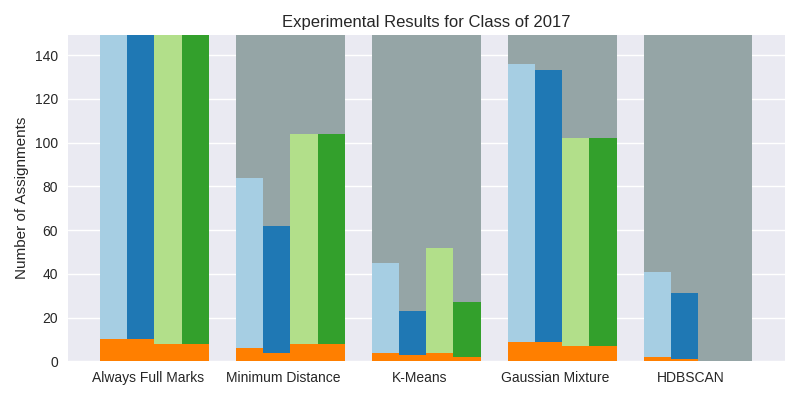
\includegraphics[width=\textwidth]{bar_triple_results_2017}
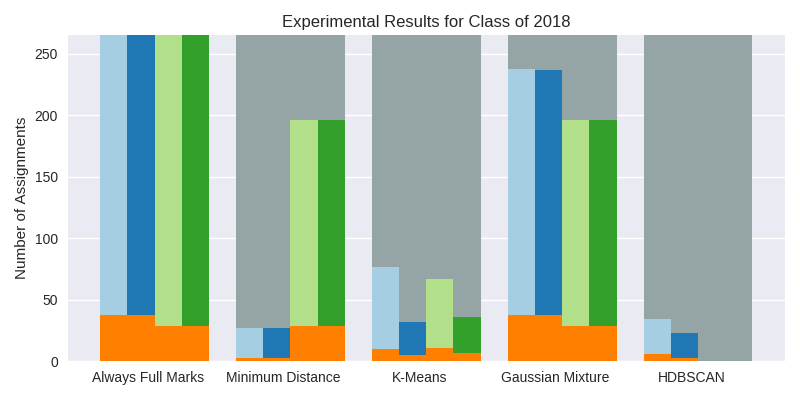
\includegraphics[width=\textwidth]{bar_triple_results_2018}
\caption[Experimental Results for Classes of 2017 and 2018]{These graphs break down the outcomes of the assignments for each class. The grey bars represent the number of assignments that must be manually marked; the light blue and dark blue bars represent the number of automated Non-Blocking IO assignments at the 90 and 95 cutoffs, respectively; similarly, the green bars represent the Parallel Processing assignment; and finally, the orange bars represent the number of automated assignments deemed to be false positives.}
\label{fig:ctm-results}
\end{figure}

Figure~\ref{fig:ctm-results} presents our experimental results. Since Always Full Marks did not perform any analysis, it would not encounter any processing errors and thus would always be able to automate every assignment. Clearly this was the maximum possible value and could not be exceeded; the goal for the other algorithms was to automate as many assignments as possible. While near-100\% automation rate was unrealistic due to potential processing errors, we hoped to be able to automate at least half the assignments. The false positives for Always Full Marks was simply the students that did not receive full marks. Therefore, we required the other algorithms to achieve a better false positive count than this trivial approach to be considered an improvement.

Firstly, the Minimum Distance algorithm was able to achieve slightly fewer false positives than Always Full Marks with an acceptable number of automated assignments. With the exception of Non-Blocking IO in 2018, this algorithm was able to automate almost half of the classes, which would greatly reduce the time needed for manual marking.

Secondly, the K-Means algorithm was able to achieve even fewer false positives than Minimum Distance; conversely, it automated even fewer assignments. However, we note that at the 90 cutoff, K-Means was still able to automate approximately a third of the assignments, which was a non-trivial reduction in manual work for human markers.

Thirdly, the Gaussian Mixture algorithm was able to achieve the highest automation rates out of all of our proposed algorithms. However, we note that this algorithm appeared to be strictly worse than the baseline Always Full Marks because its number of false positives was on par with the baseline despite not being able to automate as much.

Fourthly, the HDBSCAN algorithm was able to achieve the lowest number of false positives; conversely, it automated the fewest assignments. In addition, it appeared to be unable to flag any correct Parallel Processing solutions for the 2018 class; since this was exclusive to one class and not both, we believe this may have been due to minor assignment specification changes over the years and that our reference solutions were not up-to-date.

Finally, one common observation for all the graphs was that increasing the cutoff point decreased both the number of automated assignments and false positives. This was expected because a higher cutoff enforced a higher confidence in our prediction, i.e. the predicted score must be within 5 points of 100 to be considered correct instead of 10 points. Naturally, with a stricter requirement, the number of assignments that we could automate and the number of false positives also decreased.
